\RussianSourceFrame{GELFAND-P001415}{unlabelled}
(15) \underline{Теорема}. Пусть $\lambda$ — диаг. из $N$ элементов и
$q\ne\sqrt[m]{1}$. Тогда $S_{\lambda}^{(k)}$ задают представление алгебры Гекке
(в образующих $e_k$).

Построим ф-и $W$.
$W_{-r}(\tau)$ при $r=1,2,\ldots$ опред. из соотношений
\begin{equation}
 W_{-(r+1)}(\tau)=1-\frac{\tau}{W_{-r}(\tau)},\qquad r\geq0,
 \tag{16}
\end{equation}
[Зачёркнуто: \RussianUnclear{GELFAND-P001415}{eq16-cancelled}{а при $r\ne0$; возможно, $r\geq0$.}]
\begin{equation}
 W_r(\tau)=1-W_{-r}(\tau),\qquad r\geq0;
 \tag{17}
\end{equation}

Или:

$W_{-r}(\tau)$ опр.
[Зачёркнуто: \RussianUnclear{GELFAND-P001415}{continued-fraction-cancelled-word}{неразборчиво}]
из разл. в цепную дробь:
\begin{equation}
 \text{[Зачёркнуто: }W_{-r}(\tau)=\text{]}\quad
 1-\frac{\tau}{1-\dfrac{\tau}{1-\ldots}}
 \tag{18}
\end{equation}
Имеется ур-е:
\begin{equation}
 W_r(\tau)W_{1-r}(\tau)=1.
 \tag{19}
\end{equation}
\RussianUnclear{GELFAND-P001415}{eq19-right-hand-side}{В правой части написано $1$.}

Общая ф-ла:
\begin{equation}
 W_r(\tau)=\frac{q(q^{r-1}-1)}{(q+1)(q^r-1)},\qquad r=1,2,\ldots
 \tag{20}
\end{equation}
\begin{equation}
 W_{-r}(\tau)=\frac{q^{r+1}-1}{(q+1)(q^r-1)}.
 \tag{21}
\end{equation}
\RussianUnclear{GELFAND-P001415}{w-index}{Индекс функций $W$: $r$; возможно, $i$.}

(22) \underline{Задача}: найти характеры алгебры Гекке.

Рассмотрим
\begin{equation}
 \frac{
 \begin{vmatrix}
 x_1^{i_1}&x_1^{i_2+1}&\ldots&x_1^{i_n+n-1}\\
 x_2^{i_1}&x_2^{i_2+1}&\ldots&x_2^{i_n+n-1}\\
 \ldots&\ldots&\ldots&\ldots\\
 x_n^{i_1}&\ldots&\ldots&x_n^{i_n+n-1}
 \end{vmatrix}
 }{
 \begin{vmatrix}
 1&x_1&x_1^2&\ldots&x_1^{n-1}\\
 1&x_2&x_2^2&\ldots&\\
 \ldots&\ldots&\ldots&\ldots&\\
 1&x_n&x_n^2&\ldots&x_n^{n-1}
 \end{vmatrix}
 }
 =\sum a(i,j)P_{j_1}P_{j_2}\ldots P_{j_n}
 \tag{23}
\end{equation}
\RussianUnclear{GELFAND-P001415}{eq23-overwritten-exponents}{В первых двух строках последнего столбца числителя: $i_n+n-1$; нижний индекс у $i$ исправлен поверх прежних штрихов.}


\RussianSourceFrame{GELFAND-P001416}{53}
$j=(j_1,\ldots,j_n)$, $P_j$ — сумма степеней.

Тогда

(24) $a(i,j)$ — знач. характера [вставлено над строкой: симм. группы]
на элем. с длинами циклов $j_1,\ldots,j_n$

(с точн. до простой константы)

По поводу симм. группы см. книгу Макдональда «Симм. ф-и
и многочлены Холла».

\medskip
\underline{Локализация полюсов у дзета-функции Рюэлля.}

(\RussianUnclear{GELFAND-P001416}{mayer-name}{Линдон Майер (?)})

Letters in Math. Physics, $14:2$, 1987 г.

$I$ — интервал, $T:I\to I$ — кусочно линейное
\begin{equation*}
 I=\bigcup_j I_j,\qquad T(I_j)=I.
\end{equation*}
\RussianSourceFigure{GELFAND-P001416}{interval-graph}{Прямоугольная рамка без подписей; внутри несколько восходящих наклонных ветвей и почти вертикальных штрихов. Принадлежность коротких штрихов ветвям и точное число разрывов требуют сверки с оригиналом.}

\begin{center}
\begin{minipage}[t]{.46\linewidth}\vspace{0pt}\centering
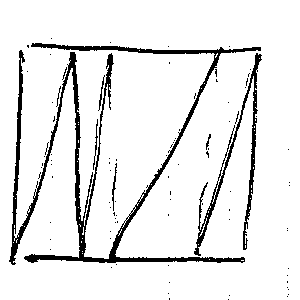
\includegraphics[width=\linewidth]{figures/gelfand-0154-p001416-interval-graph-original.png}\par\smallskip
{\footnotesize Оригинал рукописного рисунка: \texttt{GELFAND-P001416}}
\end{minipage}\hfill
\begin{minipage}[t]{.50\linewidth}\vspace{0pt}\centering
{\footnotesize Частичное воссоздание видимых штрихов}\par\smallskip
\resizebox{\linewidth}{!}{% Visible strokes only. Coordinate scale reproduces the sketch, not an exact map.
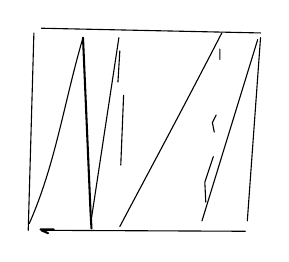
\begin{tikzpicture}[x=.012cm,y=-.012cm,line cap=round]
\draw (20,50)--(14,259) (28,45)--(260,50) (260,55)--(246,249)
 (31,259)--(244,260);
\draw (15,252) .. controls (43,189) and (52,123) .. (72,55);
\draw[line width=.75pt] (72,55)--(80,240)--(81,257);
\draw (81,246)--(110,55);
\draw (111,69)--(109,102) (115,116)--(112,190);
\draw (111,255) .. controls (140,200) and (171,143) .. (219,50);
\draw (198,249)--(257,57);
\draw (202,229)--(201,208)--(210,181) (211,155)--(209,145)--(213,137)
 (217,67)--(217,78);
% The thick bottom-left terminal trace is not interpreted as an arrow.
\draw[line width=.75pt] (27,258)--(41,258) (28,259)--(35,262);
\end{tikzpicture}
}
\end{minipage}
\end{center}
\noindent{\small\textit{Открытые соединения и короткие вертикальные штрихи остаются неустановленными после просмотра при 3×, 5× и 10×. Простые линии не задают стрелок, разрывов или дополнительных значений осей.}}


\begin{equation}
 \zeta_T(z,\varphi)=\frac{\det(1-zL_1)}{\det(1-zL_2)},
 \tag{1}
\end{equation}
где
\begin{equation*}
 L_1f(z)=\varphi(z)\sum\frac{1}{\rho_j}f(\psi_j(z)),
\end{equation*}
\begin{equation*}
 L_2f(z)=\varphi(z)\sum f(\psi_j(z)),
\end{equation*}
$\psi_j$ — локальные обратные $T$ на интервале $I_j$, а $\rho_j^{-1}$ — наклон.
\RussianUnclear{GELFAND-P001416}{slope-letter}{Буква в $\rho_j$ допускает также чтение $p_j$.}

В общем случае:
\begin{equation}
 \zeta_T(z,\varphi)=
 \exp\left(
 \sum_{n=1}^{\infty}\frac{z^n}{n}
 \sum_{\xi\in\mathrm{Fix}\,T^n}
 \prod_{k=0}^{n-1}\varphi(T^k x)
 \right)
 \tag{2}
\end{equation}
\RussianUnclear{GELFAND-P001416}{eq2-variable}{Под второй суммой написано $\xi\in\mathrm{Fix}\,T^n$, в произведении — $x$.}


\RussianSourceFrame{GELFAND-P001417}{unlabelled}
\underline{7/XII-87.}\qquad \underline{Сем. Гельфанда!}\qquad Нечто о работе

\underline{D. Mayer}\qquad \underline{Lett. in Math. Phys. 1987, $14:2$}

\underline{О $\zeta$-функции Рюэлля}

$F$ — мн-во значений спина (конечное).

Изучаем конфигурации спина на решётке
\begin{equation*}
 (\xi_i),\qquad -\infty<i<\infty,\qquad \xi_i\in F.
\end{equation*}
$M\subseteq F\times F$ — допустимое мн-во; требуется, чтобы было
\begin{equation}
 (\xi_i,\xi_{i+1})\in M.
 \tag{1}
\end{equation}

Простейший пример рюэллевской $\zeta$-ф-и — $\zeta$-ф-я Артина и Мазура.

Рассм. мн-во периодических конфигураций и их количество:
\begin{equation}
 N_n=\#\{(\xi_i)\mid\mathcal T^n(\xi_i)=(\xi_i)\}
 =\mathrm{Fix}\,\mathcal T^n,
 \tag{2}
\end{equation}
где $\mathcal T$ — преобр. в пр-ве послед.
\begin{equation*}
 \mathcal T(\xi_i)=\xi_{i+1}
\end{equation*}
(сдвиг)

$\zeta$-ф-я Рюэлля:
\begin{equation}
 \zeta_{\mathcal T}(s)=\exp\left(\sum_{n=1}^{\infty}\frac{N_n}{n}s^n\right)
 \tag{3}
\end{equation}
ряд сходится при $|s|<\dfrac{1}{|F|}$.

\RussianUnclear{GELFAND-P001417}{continuation-question-overwriting}{Сущ. ли аналитическое продолжение? [Конец «Сущ.» и начальная «а» обведены поверх прежних штрихов.]}
Рассм. матрицу
\begin{equation}
 T=(T_{\alpha\beta})=
 \begin{cases}
 1,&(\alpha,\beta)\in M,\\
 0,&(\alpha,\beta)\notin M.
 \end{cases}
 \tag{4}
\end{equation}

Тогда
\begin{equation}
 \zeta_{\mathcal T}(s)=\frac{1}{\det(1-sT)}
 \tag{5}
\end{equation}

Отсюда видно, что $\zeta_{\mathcal T}(s)$ мероморфна.

Радиус сход. может быть больше, чем $1/|F|$.

Для док-ва нужно заметить, что
\begin{equation}
 N_n=\mathrm{Tr}\,T^n.
 \tag{6}
\end{equation}


\RussianSourceFrame{GELFAND-P001418}{62}
\underline{Замеч. И.М.Г.}: это похоже на раб. Дынкина и Дмитриева:
рассм. стох. матрицу $(p_{ik})$ [вставлено сверху: (стохастическую)]
(в задаче о бассейнах это
[зачёркнутый знак: \RussianUnclear{GELFAND-P001418}{basin-cancelled-sign}{неразборчиво}]
доля воды, перелив. из $i$-го басс. в $k$-й).
\begin{equation*}
 \underline{P}=(p_{ik}),\qquad \sum_k p_{ik}=1.
\end{equation*}
Это зависит от соб. значений $P$.

а) Соб. значения лежат в круге $|\lambda|\leq1$,

б) $1$ — соб. значение.

Какую обл. заполняют соб. значения?

Это внутр. нек-рой алг. кривой.

Они делали неправильно.

Есть набор соб. значений!!

и надо рисовать набор соб. значений в $\mathbb C^n$ — это должна
быть красивая область (\underline{Задача!!})

Проекция на одну ось может быть сложной!

[Слева двойная черта; следующие две строки подчёркнуты:]
\underline{В задаче Рюэлля интересно посмотреть все соб. значения}

\underline{матрицы $T$.}

\medskip
\underline{Докладчик}. Обобщение примера (3)
\begin{equation}
 \zeta_{\mathcal T}(s;\varphi)=
 \exp\left(
 \sum_{n=1}^{\infty}\frac{s^n}{n}
 \sum_{\xi\in\mathrm{Fix}(\mathcal T^n)}
 \prod_{\ell=0}^{n}\varphi(\mathcal T^\ell\xi)
 \right)
 \tag{7}
\end{equation}
\RussianUnclear{GELFAND-P001418}{eq7-upper-product-bound}{Верхний предел произведения написан как $n$.}

Здесь
\begin{equation*}
 \varphi=\varphi(\xi_1,\ldots,\xi_k),\qquad \xi_j\in F
\end{equation*}
[Под $\varphi$ черта к подписи: функция.]

($\varphi$ берётся только от первых $k$ значений).

((3) получается при $\varphi=1$)

(8) \underline{Утв.} $\exists$ [зачёркнуто: оператор; над строкой вставлено: матрица]
$L$ (конечномерная), такая что:
\begin{equation}
 \zeta_{\mathcal T}(s,\varphi)=\frac{1}{\det(1-sL)}
 \tag{9}
\end{equation}

А именно, рассм.
\begin{equation*}
 F'=F^k;
\end{equation*}
[Зачёркнуто: \RussianUnclear{GELFAND-P001418}{before-m-prime-cancelled}{неразборчивая запись перед $M'$}.]
\begin{equation*}
 M'\subset F'\times F'
\end{equation*}
\begin{equation}
 M'=\{(\xi_1,\ldots,\xi_k);(\xi_2,\ldots,\xi_{k+1})
 \mid(\xi_i,\xi_{i+1})\in M\}
 \tag{10}
\end{equation}
\RussianUnclear{GELFAND-P001418}{eq10-overwritten-indices}{Во втором кортеже индексы $2$ и $k+1$ исправлены; в условии $i+1$ также обведён.}

Тогда надо взять
\begin{equation*}
 \ell_{\alpha\beta}=
 \begin{cases}
 \varphi(\alpha),&(\alpha,\beta)\in M',\\
 0,&(\alpha,\beta)\notin M',
 \end{cases}
 \qquad L=(\ell_{\alpha\beta}).
\end{equation*}


\RussianSourceFrame{GELFAND-P001419}{unlabelled}
\underline{И.М.Г.:}

\underline{NB}: надо знать $p$-адич. числа

(уметь их складывать, умножать, делить,
[зачёркнуто: \RussianUnclear{GELFAND-P001419}{nb-cancelled-letter}{неразборчивый знак}]
извлекать корни!)

\medskip
\underline{Бейлинсон А.}\qquad
\underline{$p$-адические числа и физика.}

\underline{О каких-то $p$-адических идеях Манина в области физики}
\RussianUnclear{GELFAND-P001419}{heading-last-sign}{!; возможно, ?}

$1^{\circ}$. Виттен слушал доклад
\RussianUnclear{GELFAND-P001419}{faltings-name}{Фалтинса}
с большим интересом, после чего купил все книги по теории чисел.
Единств., что он понял из доклада — это ф-ла
\begin{equation}
 |a|_\infty\cdot|a|_2|a|_3\ldots=1,\qquad a\in\mathbb Q.
 \tag{1}
\end{equation}
Для $\dfrac12$ здесь стоит:
\begin{equation*}
 \frac12\cdot2\cdot1\ldots=1.
\end{equation*}

Есть 3 статьи:

1) \underline{Волович}\qquad (по-русски)

2) \underline{Ю.И. Манин}\qquad (по-английски)

3) \underline{Witten} и кто-то ещё
\RussianUnclear{GELFAND-P001419}{witten-list-final-sign}{[неразборчивый отдельный знак после строки]}

Все 3 статьи появились в сентябре.

\underline{Текст Виттена.}

Рассм. функц. ур-е для $\zeta$-ф-и Римана
\begin{equation}
 \pi^{-s/2}\Gamma(s/2)\prod(1-p^{-s})^{-1}
 =
 \pi^{-(1-s)/2}\Gamma\left(\frac{1-s}{2}\right)
 \prod(1-p^{-(1-s)})^{-1}.
 \tag{2}
\end{equation}
(аналит. продолжение подразумевается)

или (формально):
\begin{equation}
 \frac{\pi^{-s+1}\Gamma(s/2)}
 {\Gamma\left(\dfrac{1-s}{2}\right)}
 =
 \prod_p\frac{1-p^{-s}}{1-p^{s-1}}.
 \tag{3}
\end{equation}
\RussianUnclear{GELFAND-P001419}{eq3-pi-exponent}{Показатель степени $\pi$ написан как $-s+1$.}

Слева $\approx$ амплитуда Венециано–Виттена для открытой
струны [вставлено сверху: (с импульсом $s$)].
Справа расходящееся выражение, но важно,
что она представлена в виде произведения по простым числам!


\RussianSourceFrame{GELFAND-P001420}{63}
\underline{$2^{\circ}$. О раб. Манина}

(1) \underline{Утверждение}: Мера Тамагавы $=1$.

Подробнее:
\begin{equation*}
 \mathrm{SL}(n,\mathbb R)\supset\mathrm{SL}(n,\mathbb Z).
\end{equation*}
На $\mathrm{SL}(n,\mathbb R)$ есть инвар. мера (стандартная)
[над «инвар.» вставлено: лево].

Нормируем [зачёркнуто:
\RussianUnclear{GELFAND-P001420}{normalization-cancelled}{неразборчиво}]
за счёт целочисл. матриц.
\begin{equation*}
 \operatorname{vol}\bigl(\mathrm{SL}(n,\mathbb R)/\mathrm{SL}(n,\mathbb Z)\bigr)-?
\end{equation*}

[На правом поле:]
(строится по станд. базису в алгебре Ли
$\mathfrak{sl}(n,\mathbb R)$ или в $\mathfrak{gl}(n,\mathbb R)$
[зачёркнуто: \RussianUnclear{GELFAND-P001420}{margin-cancelled}{неразборчивый знак}]
станд. базис;
\begin{center}
 \fbox{$\operatorname{vol}_{sl}=\dfrac{\operatorname{vol}_{gl}}{d\,\operatorname{tr}}$}
\end{center}
\RussianUnclear{GELFAND-P001420}{margin-volume-formula}{Формула на поле: $\operatorname{vol}_{sl}=\operatorname{vol}_{gl}/d\,\operatorname{tr}$; малые буквы у $\operatorname{vol}$ требуют сверки.}

$\mathrm{SL}(2,\mathbb R)$ — конф. преобр. ед. круга, транзит. действ.
на $S^*H^2$.

Инвар. объём на $S^*H^2$ есть
[зачёркнуто: \RussianUnclear{GELFAND-P001420}{invariant-volume-cancelled}{неразборчивый знак}]
$\operatorname{vol}_{H^2}\otimes d\varphi$.

\begin{center}
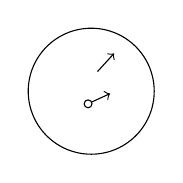
\begin{tikzpicture}[x=1cm,y=1cm]
 \draw (0,0) circle (0.8);
 \draw (-0.04,-0.16) circle (0.05);
 \draw[->] (0,-0.14) -- (0.24,-0.03);
 \draw[->] (0.08,0.25) -- (0.29,0.48);
\end{tikzpicture}
\end{center}

Или: профакторизовать по max комп. подгруппе

\begin{center}
\begin{tikzpicture}[x=1cm,y=1cm]
 \draw (0,0) circle (1.15);
 \draw (0.05,1.14) .. controls (0.08,0.65) and (-0.01,0.2) .. (-0.39,-0.12);
 \draw (0.05,1.14) .. controls (0.04,0.62) and (0.27,0.42) .. (0.43,0.10);
 \draw (-0.39,-0.12) .. controls (-0.05,0.17) and (0.23,0.17) .. (0.43,0.10);
 \draw (0.045,0.72) -- (0.19,0.66);
 \draw (-0.27,0.02) .. controls (-0.2,0.03) .. (-0.18,0.12);
 \draw (0.32,0.12) .. controls (0.27,0.18) .. (0.30,0.27);
 \node at (0.11,0.52) {$0$};
 \draw (2.8,1.1) .. controls (2.7,0.38) and (2.45,0.02) .. (1.89,-0.32);
 \draw (2.8,1.1) .. controls (2.77,0.48) and (3.11,0.09) .. (3.46,-0.35);
 \draw (1.89,-0.32) .. controls (2.39,-0.12) and (2.98,-0.06) .. (3.46,-0.35);
 \draw (2.69,0.68) -- (2.84,0.7);
 \draw (2.17,-0.16) .. controls (2.29,-0.1) .. (2.30,0.03);
 \draw (3.17,-0.19) .. controls (3.12,-0.10) .. (3.14,0.02);
 \node at (2.78,0.51) {$0$};
 \node at (2.43,0.04) {$\pi/3$};
 \node at (3.04,0.03) {$\pi/3$};
 \draw[->] (4.05,0.49) -- (3.59,0.49);
 \node[anchor=west] at (4.13,0.49) {\underline{фунд. область}};
\end{tikzpicture}
\end{center}

\underline{Ответ.}
\begin{equation}
 \operatorname{vol}\mathrm{SL}(n,\mathbb R)/\mathrm{SL}(n,\mathbb Z)
 =\zeta(2)\zeta(3)\ldots\zeta(n)
 \tag{2}
\end{equation}
$\mathbb A$ — адели;
\begin{equation}
 \begin{gathered}
 \mathrm{SL}(n,\mathbb A)\sim
 \mathrm{SL}(n,\mathbb R)\times\mathrm{SL}(n,\mathbb Q_2)\times\ldots\\
 \cup\\
 \mathrm{SL}(n,\mathbb Q)
 \end{gathered}
 \tag{3}
\end{equation}
\begin{equation}
 \operatorname{vol}\mathrm{SL}(n,\mathbb A)/\mathrm{SL}(n,\mathbb Q)=1.
 \tag{4}
\end{equation}
\begin{equation*}
 \operatorname{vol}\mathrm{SL}(n,\mathbb A)/\mathrm{SL}(n,\mathbb Q)
 \sim
 \operatorname{vol}\mathrm{SL}(n,\mathbb R)/\mathrm{SL}(n,\mathbb Z)
 \prod\operatorname{vol}\mathrm{SL}(n,\mathbb Z_p).
\end{equation*}
\begin{equation}
 \operatorname{vol}\mathrm{SL}(n,\mathbb Z_p)
 \sim\#\mathrm{SL}_n(\mathbb F_p)/p^{n^2-1}.
 \tag{5}
\end{equation}
\underline{Упражнение}: вычислить $\#\mathrm{SL}_n(\mathbb F_p)$.


\RussianSourceFrame{GELFAND-P001421}{unlabelled}
(6) Число элем. $\mathrm{GL}(n,\mathbb F_p)$
\begin{equation*}
 (p^n-1)(p^n-p)(p^n-p^2)\ldots
 =
 p^{n^2}(1-p^{-n})(1-p^{-n+1})\ldots(1-p^{-1}).
\end{equation*}

(7) Для $\mathrm{SL}(n,\mathbb F_p)$ надо поделить на $p-1$:
\begin{equation*}
 p^{n^2-1}(1-p^{-n})(1-p^{-n+1})\ldots(1-p^{-2}).
\end{equation*}
Это произвед. эйлеровых сомножителей.

(8) \underline{Гипотеза Ю.И. Манина}: аналог ф-лы (2) можно написать для
пр-в модулей кривых, возник. в теории струн.

\underline{И.М.Г.}

\underline{Мат. вопрос}: объём пр-ва Тейхмюллера имеет $p$-адический аналог.

Или: что такое адельное пр-во Тейхмюллера

\medskip
\underline{Пример \RussianUnclear{GELFAND-P001421}{witten-heading-faint-word}{силы} работ Виттена:}

\underline{Laumon} сделал раб. по теории чисел на основе идей Виттена
из теории Морса.

Идея: рассм. ф-ю $u\in\mathcal E'(\mathbb R)$,
$\widetilde u(\xi)\in C^\infty$
и все особ. уйдут в асимптотику на бесконечности.

\underline{Совет И.М.Г.}: прочитать книгу Харкевича
«Спектры, [зачёркнуто:
\RussianUnclear{GELFAND-P001421}{book-title-cancelled}{неразборчиво};
вставлено над строкой: сигналы] и шумы»,
чтобы понимать преобр. \underline{Фурье}.

О раб. \underline{Laumon'а}.

\begin{center}
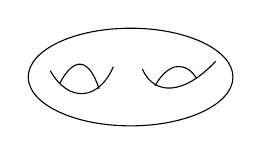
\begin{tikzpicture}[x=1cm,y=1cm]
 \draw (0,0) ellipse (1.3 and 0.62);
 \draw (-1.02,0.08) .. controls (-0.78,-0.34) and (-0.40,-0.29) .. (-0.22,0.13);
 \draw (-0.90,-0.08) .. controls (-0.72,0.26) and (-0.53,0.25) .. (-0.40,-0.15);
 \draw (0.15,0.10) .. controls (0.30,-0.24) and (0.68,-0.23) .. (1.08,0.20);
 \draw (0.31,-0.11) .. controls (0.50,0.22) and (0.72,0.18) .. (0.84,-0.02);
\end{tikzpicture}
\end{center}

Рассм. поверхность $\mathcal F$
\begin{equation*}
 H^i(X,\mathcal F),\qquad i=0,1,2.
\end{equation*}
\RussianUnclear{GELFAND-P001421}{surface-symbol}{После «поверхность» стоит $\mathcal F$; далее написано $H^i(X,\mathcal F)$.}

\begin{equation}
 \det H^\bullet(X,\mathcal F)=
 \frac{\det H^0(X,\mathcal F)\det H^2(X,\mathcal F)}
 {\det H^1(X,\mathcal F)\;
 \text{[зачёркнуто: }\det H^2(X,\mathcal F)\text{]}}
 \tag{1}
\end{equation}
([Зачёркнуто:
\RussianUnclear{GELFAND-P001421}{before-vector-spaces-cancelled}{конечные?}]
вект. пр-ва;
$\det$ — max внеш. степень)

Автоморфизмы?

Рассм. триангуляцию; $\det H^\bullet$ отожд. с произвед. $\det$
членов комплекса (ф-ла типа Эйлера): канонически


\RussianSourceFrame{GELFAND-P001422}{64}
\begin{equation*}
\det(C^\bullet)=\det(H^\bullet(C)) \tag{2}
\end{equation*}
$2-2g$ — эйлерова хар-ка.

С другой стороны
\begin{equation*}
2g-2=\operatorname{deg}K
\end{equation*}
[Под $K$: «кан. класс».]

\underline{Пусть}

$D$ — дивизор;
\begin{equation*}
\det\mathcal F_D=\bigotimes(\det\mathcal F_{x_i})^{\otimes a_i},
\qquad D=\sum a_i x_i \tag{3}
\end{equation*}
[Зачёркнуто:
\RussianUnclear{GELFAND-P001422}{cancelled-divisor-map}{$D\to D+K$ или $D\mapsto D+K$; чтение не установлено}.]

\underline{Ф-ла Делиня:}
\begin{equation*}
\det H^\bullet=\det\mathcal F_K \tag{4}
\end{equation*}
[Справа зачёркнут отдельный знак:
\RussianUnclear{GELFAND-P001422}{eq4-cancelled-sign}{неразборчиво}.]
\RussianUnclear{GELFAND-P001422}{eq4-determinant-convention}{В (4) написано $\det H^\bullet=\det\mathcal F_K$, без показателя $-1$.}

(фиксир. комплексную структуру и выбор точки в кан. классе)

Для произв. конструкт. пучка тоже считается $\underline{\det}$ и
есть аналог ф-лы Делиня!

Здесь на $\mathbb A^1$ возникают ф-и с особенностями

\underline{\underline{Клячко.}}\quad
\underline{\underline{Торические расслоения.}}

Торическое мн-зие — мн-зие $X$ на к-ром действует алг. тор $T$;
причём есть орбита, изом. $T$.
\begin{equation*}
X=\bigcup_\sigma O_\sigma,\quad\text{— разложение на орбиты}
\end{equation*}
$\mathcal E$ — расслоение на $X$ с торической структурой
(и действие поднимается! диагр.
\begin{equation*}
\begin{tikzcd}
\mathcal E \arrow[r,"t"] \arrow[d] & \mathcal E \arrow[d] \\
X \arrow[r,"t"] & X
\end{tikzcd}
\end{equation*}
коммутативна)

Можно описать модули [вставлено над строкой: «таких»]
расслоений на языке линейной алгебры.


\RussianSourceFrame{GELFAND-P001423}{unlabelled}
Строение $X$ описывается веером $\Sigma$ в алгебре Ли тора.
\begin{center}
\begin{tikzpicture}[scale=0.9]
\draw (0,0) -- (-1.65,0.9);
\draw (0,0) -- (-1.45,-0.95);
\draw (0,0) -- (-0.12,1.65);
\draw (0,0) -- (0.15,-1.65);
\draw[->] (0,0) -- (1.05,1.45);
\draw[->] (0,0) -- (1.8,0.9);
\draw[->] (0,0) -- (1.85,-0.5);
\draw (0.36,0.19) -- (0.3,0.42);
\draw (0.64,0.32) -- (0.52,0.72);
\draw (0.95,0.48) -- (0.76,1.05);
\draw (1.28,0.64) -- (1.02,1.33);
\draw (0.35,-0.10) -- (0.43,0.20);
\draw (0.64,-0.18) -- (0.71,0.33);
\draw (0.96,-0.26) -- (1.03,0.47);
\draw (1.29,-0.35) -- (1.35,0.59);
\node at (1.65,1.35) {$\sigma$};
\node at (1.95,0.28) {$\sigma$};
\node at (4.3,0.75) {(конусы)};
\end{tikzpicture}
\end{center}
$|\Sigma|$ — мн-во $1$-мерных конусов в веере $\Sigma$.

\underline{Теорема.}
(Катег. торич. расслоений) $\Longleftrightarrow$
(катег. вект. пр-в
[зачёркнут знак:
\RussianUnclear{GELFAND-P001423}{theorem-cancelled-sign}{неразборчиво}]
$E$ набором [над строкой вставлено: «убыв. $\mathbb Z$-»]
фильтраций $E^\alpha(i)$, $\alpha\in|\Sigma|$, удовл. условию

А) Фильтрации $E^\alpha$, $\alpha\in\sigma\in\Sigma$,
дистрибутивны.

\underline{Задачи.}
1) Описать геометрию расслоения (когом., хар. классы
и т. п.) на языке фильтраций

2) классификация — ?

Пусть $\Sigma$ — симплиц. комплекс; поставим вершине в соотв.
фильтрацию

Его предст. — набор фильтраций в вект. пр-ве
[вставлено над строкой: «$E$:»] $E^\alpha(i)$,
$\alpha\in$ [зачёркнут знак:
\RussianUnclear{GELFAND-P001423}{representation-cancelled-sign}{неразборчиво}]
$\Sigma$,
\begin{equation*}
E\ldots\supset E^\alpha(i)\supset E^\alpha(i+1)\supset\ldots 0
\end{equation*}
\begin{equation*}
\alpha\in(\text{вершины комплекса})=\Sigma.
\end{equation*}
Пр-ва $E^\alpha(i)$, $\alpha\in\sigma$, дистрибутивны при фиксир. $\sigma$
(для всех $i$)

[Под первым $\sigma$: «симплекс». Вставка в обводке:]
(т. е. порождают дистрибу. решётку)

Напр., если

$\alpha_1,\alpha_2,\alpha_3$ — вершины $\Delta$-ка, то

$E^{\alpha_1}\quad E^{\alpha_2}\quad E^{\alpha_3}$ дистрибутивны, т. е.
\begin{equation*}
(E^{\alpha_1}+E^{\alpha_2})\cap E^{\alpha_3}
=E^{\alpha_1}\cap E^{\alpha_3}+E^{\alpha_2}\cap E^{\alpha_3}
\end{equation*}

\underline{Классифицировать:} хорошая задача

Для тр-ка: решается тривиально

Для поверхности тетраэдра $\Sigma=\partial\Delta$, $\Delta$ — симплекс, ответ
таков: в [зачёркнуто:
\RussianUnclear{GELFAND-P001423}{tetrahedron-cancelled-space}{$\mathbb R^3$-пр-ве; чтение не установлено}]
$E$, $\dim E=3$, рассм. $4$ $2$-мерных подпр-ва общего положения.
\begin{equation*}
\mathcal E=(E;\ E^\alpha,E^\beta,E^\gamma,E^\delta)
\end{equation*}


\RussianSourceFrame{GELFAND-P001424}{65}
ещё нужно взять внешние степени
\begin{equation*}
\Lambda^i\mathcal E=
(\Lambda^i E,\Lambda^i E^\alpha,\Lambda^i E^\beta,
\Lambda^i E^\gamma,\Lambda^i E^\delta)
\end{equation*}
Общее предст. разл. в прямую сумму $1$-мерных и таких.

\underline{И. М. Г.}
Правильная задача: выделить в $\forall$ задаче разрешимые
куски (идеология Гельф.-Пономарева)

У В. [исправленный и зачёркнутый инициал:
\RussianUnclear{GELFAND-P001424}{kac-initial}{неразборчиво}]
\underline{Каца} всё это описано на языке графов и алгебр
\underline{Каца-Муди}:
размерности вершин = коорд. корней и т. п.

Находится число параметров.

Lect. Notes, \underline{996}; более ранняя раб. — \underline{Inventiones}.

(докл. на конференции)

[Зачёркнута строка:
\RussianUnclear{GELFAND-P001424}{cancelled-seminar-line}{Семинар \ldots; остальное неразборчиво}.]

\RussianIncomplete{GELFAND-P001424}{cancelled-seminar-content}{Полное чтение зачёркнутой строки перед «След. раз: 8 февраля» не установлено; возможное начальное слово приведено выше.}

\underline{След. раз:}\quad \underline{8 февраля.}

